\chapter{Codigo}

\section{Problem}


\subsubsection{Knapsack problem}

La función \ref{lst:kp-gi} genera de manera aleatoria un conjunto de elementos en la mochila con pesos y valores aleatorios en un rango de $[1,10]$. La función \ref{lst:kp-e} calcula la energía del sistema la cual suma todos los pesos y valores de los elementos que se encuentran en la solución, si el peso es menor al capacidad de la mochila entonces devuelve el valor de la mochila, en caso contrario devuelve la diferencia de el peso actual menos la capacidad máxima.

La función \ref{lst:kp-gis} genera soluciones aleatorias de combinaciones y no regresa ninguna de ellas hasta que el peso de la solución sea menor a la capacidad máxima. Finalmente, la función \ref{lst:kp-rn} se encarga de generar un vecino de forma aleatoria, primero selecciona un elemento aleatorio del vector y después lo invierte.  

\begin{lstlisting}[style=pythonstyle, label={lst:kp-gi} ,caption={Función \textit{generate\_information} de Knapsack problem}]
	def generate_information(self, items, capacity):
	self.information = {
		"items": items,
		"values": [(random.randint(1,10), random.randint(1, 10)) for _ in range(items)],
		"capacity": capacity
	}
\end{lstlisting}

\begin{lstlisting}[style=pythonstyle, label={lst:kp-e} ,caption={Función \textit{energy} de Knapsack problem}]
	def energy(self, solution, information):
	total_weight = total_value = 0
	for i in range(len(solution)):
	if solution[i] == 1:
	total_weight += information['values'][i][0]
	total_value += information['values'][i][1]
	
	if total_weight > information['capacity']:
	return information['capacity'] - total_weight
	return total_value
\end{lstlisting}

\begin{lstlisting}[style=pythonstyle, label={lst:kp-gis} ,caption={Función \textit{generate\_initial\_solution} de Knapsack problem}]
	def generate_initial_solution(self, information):
	while True:
	solution = [random.randint(0,1) for _ in information['values']]
	if self.energy(solution, information) > 0:
	return solution
\end{lstlisting}


\begin{lstlisting}[style=pythonstyle, label={lst:kp-rn} ,caption={Función \textit{random\_neighbour} de Knapsack problem}]
	def random_neighbour(self, solution):
	neighbour = solution[:]
	index = random.randint(0, len(solution) - 1)
	neighbour[index] = not neighbour[index]
	return neighbour     
\end{lstlisting}

La interfaz de la figura \ref{fig:kp} simula 125 elementos generados de forma aleatorio para ser metidos en una mochila 200 de capacidad. En verde son los objetos que están en la prueba actual de la mochila y en gris los que no. Adicionalmente se utiliza un cuadrado verde para validar que el peso actual sea menor que la capacidad máxima de la mochila.

\begin{figure}[h!]
	\centering
	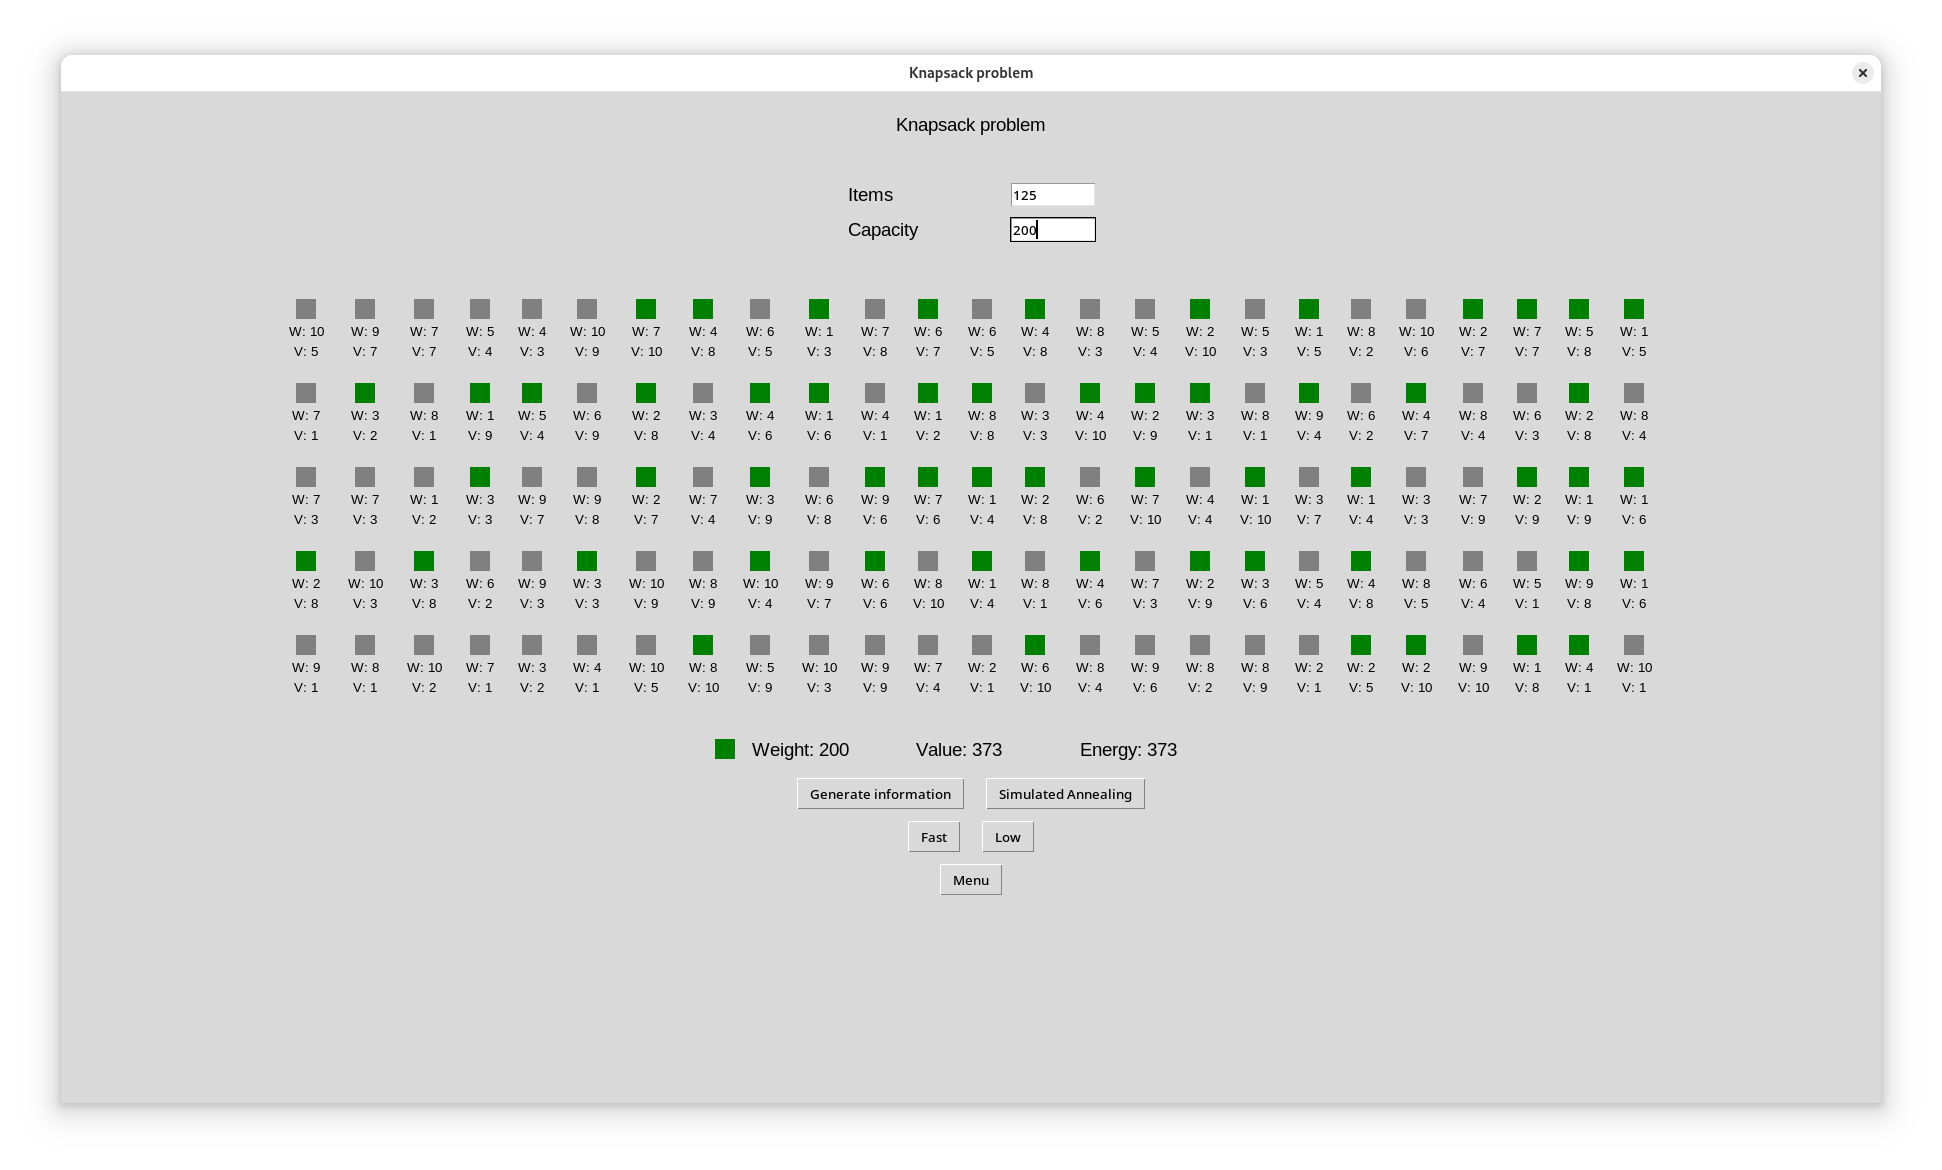
\includegraphics[width=\linewidth]{img/kp}
	\caption{Knapsack Problem Interface}
	\label{fig:kp}
\end{figure}

\subsection{Travel Salesman Problem}

La función \ref{lst:tsp-gi} genera una matriz cuadrada y simétrica de $n$ valores aleatorios en un rango de $[1, 100]$.

La función \ref{lst:tsp-e} calcula la energía del sistema. Dado un vector suma todas las distancias de las ciudades con base en la información generada en \ref{lst:tsp-gi}, el resultado que devuelve es negativo ya que se busca minimizar. La función \ref{lst:tsp-gis} genera un vector de $n$ números consecutivos (representando las ciudades) y cambia las posiciones mediante la función \textit{shuffle}.

Finalmente, la función \ref{lst:tsp-rn} toma dos indices aleatorios diferentes e invierte los valores de dichas posiciones del vector.

\begin{lstlisting}[style=pythonstyle, label={lst:tsp-gi} ,caption={Función \textit{generate\_information} de Travel Salesman Problem}]
	def generate_information(self, cities):
	distances = [[0]*cities for _ in range(cities)]
	
	for i in range(cities):
	for j in range(i, cities):  
	if i == j:
	valor = 0  
	else:
	valor = random.randint(1, 100)
	distances[i][j] = valor
	distances[j][i] = valor 
	
	self.information = {
		"cities" : cities,
		"distances" : distances
	}
\end{lstlisting}

\begin{lstlisting}[style=pythonstyle, label={lst:tsp-e} ,caption={Función \textit{energy} de Travel Salesman Problem }]
	def energy(self, solution, information):
	distance = 0
	num_cities:int = len(solution)
	
	for i in range(num_cities):
	current_city = solution[i]
	next_city = solution[(i + 1) % num_cities]  
	distance += information['distances'][current_city][next_city]
	
	return -distance
\end{lstlisting}

\begin{lstlisting}[style=pythonstyle, label={lst:tsp-gis} ,caption={Función \textit{generate\_initial\_solution} de Travel Salesman Problem}]
	def generate_initial_solution(self, information):
	solution =  list(range(information['cities']))
	random.shuffle(solution)
	return solution     
\end{lstlisting}

\begin{lstlisting}[style=pythonstyle, label={lst:tsp-rn} ,caption={Función \textit{random\_neighbour} de Travel Salesman Problem}]
	def random_neighbour(self, solution):
	neighbour = solution[:]
	i = j = random.randint(0, len(solution) - 1)
	while j == i:
	j = random.randint(0, len(solution) - 1)
	neighbour[i], neighbour[j] = neighbour[j], neighbour[i]
	
	return neighbour
\end{lstlisting}

La interfaz de la figura \ref{fig:tsp} simula 25 ciudades y muestra la exploración de diferentes posibilidades en el espacio de búsqueda. El botón de \textit{distances} muestra la matriz de adyacencia del grafo.

\begin{figure}[h!]
	\centering
	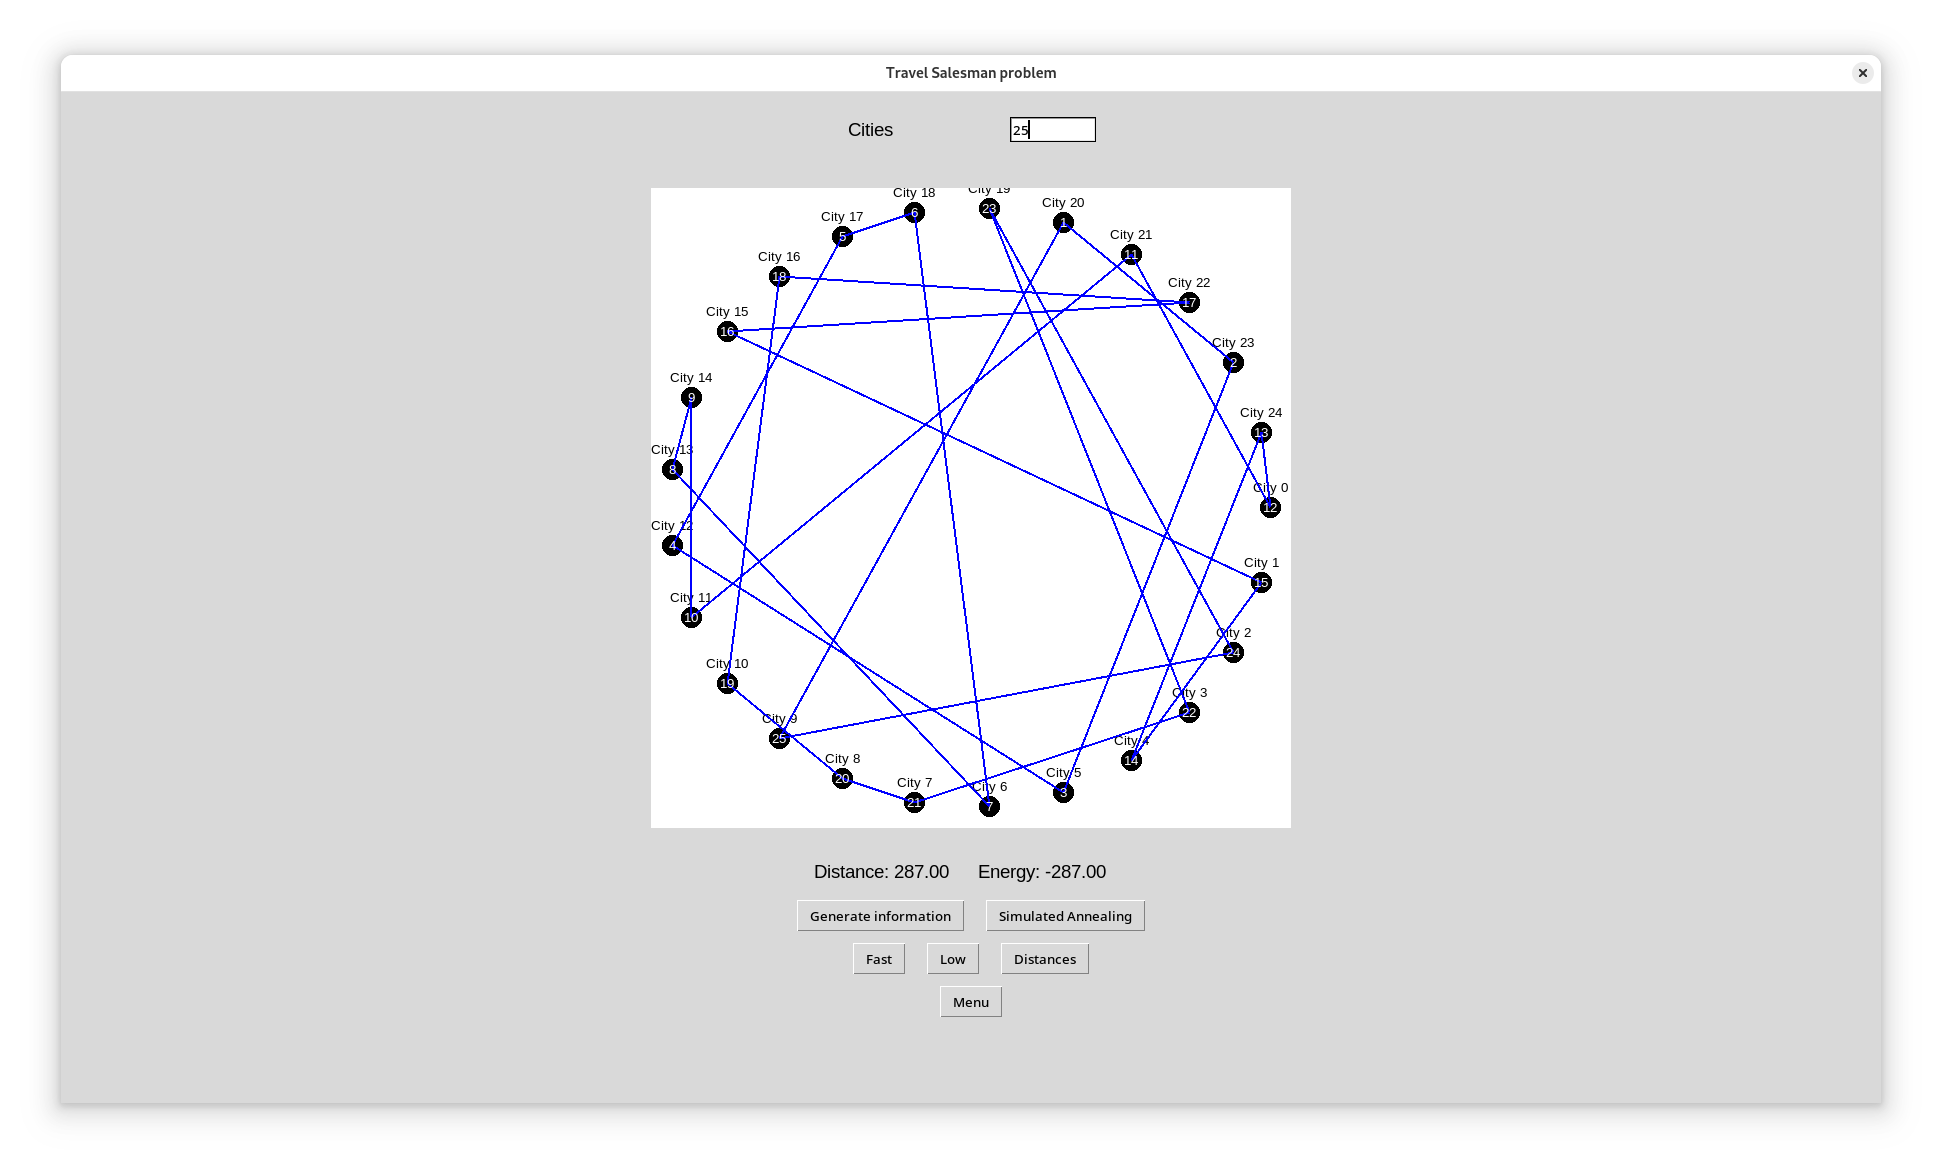
\includegraphics[width=\linewidth]{img/tsp}
	\caption{Travel Salesman Problem Interface}
	\label{fig:tsp}
\end{figure}

\subsection{Sum function Problem}

La función \ref{lst:sfp-gi} unicamente define el tamaño del vector y los rangos de valores. por otro lado, la función \ref{lst:sfp-e} calcula la energía del sistema dada por la suma de los cuadrados, dado que es una función de minimización se invierte el signo.

La función \ref{lst:sfp-gis} genera un vector de $n$ elementos aleatorios en los rangos definidos, mientras que la función \ref{lst:sfp-gn} suma  o resta en uno a un elemento aleatorio del vector (dado que se considera una configuración circular, se ajusta el valor si el nuevo valor no se encuentra en el rango).

\begin{lstlisting}[style=pythonstyle, label={lst:sfp-gi} ,caption={Función \textit{generate\_information} de SumFunctionProblem}]
	def generate_information(self, size, min, max):
	self.information = {
		"size": size,
		"min": min,
		"max": max
	}
\end{lstlisting}

\begin{lstlisting}[style=pythonstyle, label={lst:sfp-e} ,caption={Función \textit{energy} de SumFunctionProblem}]
	def energy(self, solution, _):
	total_sum:float = 0
	
	for val in solution:
	total_sum += val**2
	
	return -total_sum
\end{lstlisting}

\begin{lstlisting}[style=pythonstyle, label={lst:sfp-gis} ,caption={Función \textit{generate\_initial\_solution} de SumFunctionProblem}]
	def generate_initial_solution(self, information):
	solution = [random.randint(information['min'], information['max']) for _ in range(information['size'])]
	return solution
\end{lstlisting}

\begin{lstlisting}[style=pythonstyle, label={lst:sfp-gn} ,caption={Función \textit{generate\_neighbour} de SumFunctionProblem}]
	def random_neighbour(self, solution):
	neighbour = solution[:]
	index = random.randint(0, len(solution) - 1)
	sign = random.choice([-1 , 1])
	neighbour[index] += sign
	
	if neighbour[index] > self.information['max']:
	neighbour[index] = self.information['min']
	
	if neighbour[index] < self.information['min']:
	neighbour[index] = self.information['max']
	
	return neighbour
\end{lstlisting}

La interfaz de la figura \ref{fig:sfp} simula un vector de 30 elementos en el rango de -10 a 10. Las barras crecen y decrecen según se explore el espacio de búsqueda. 

\begin{figure}[h!]
	\centering
	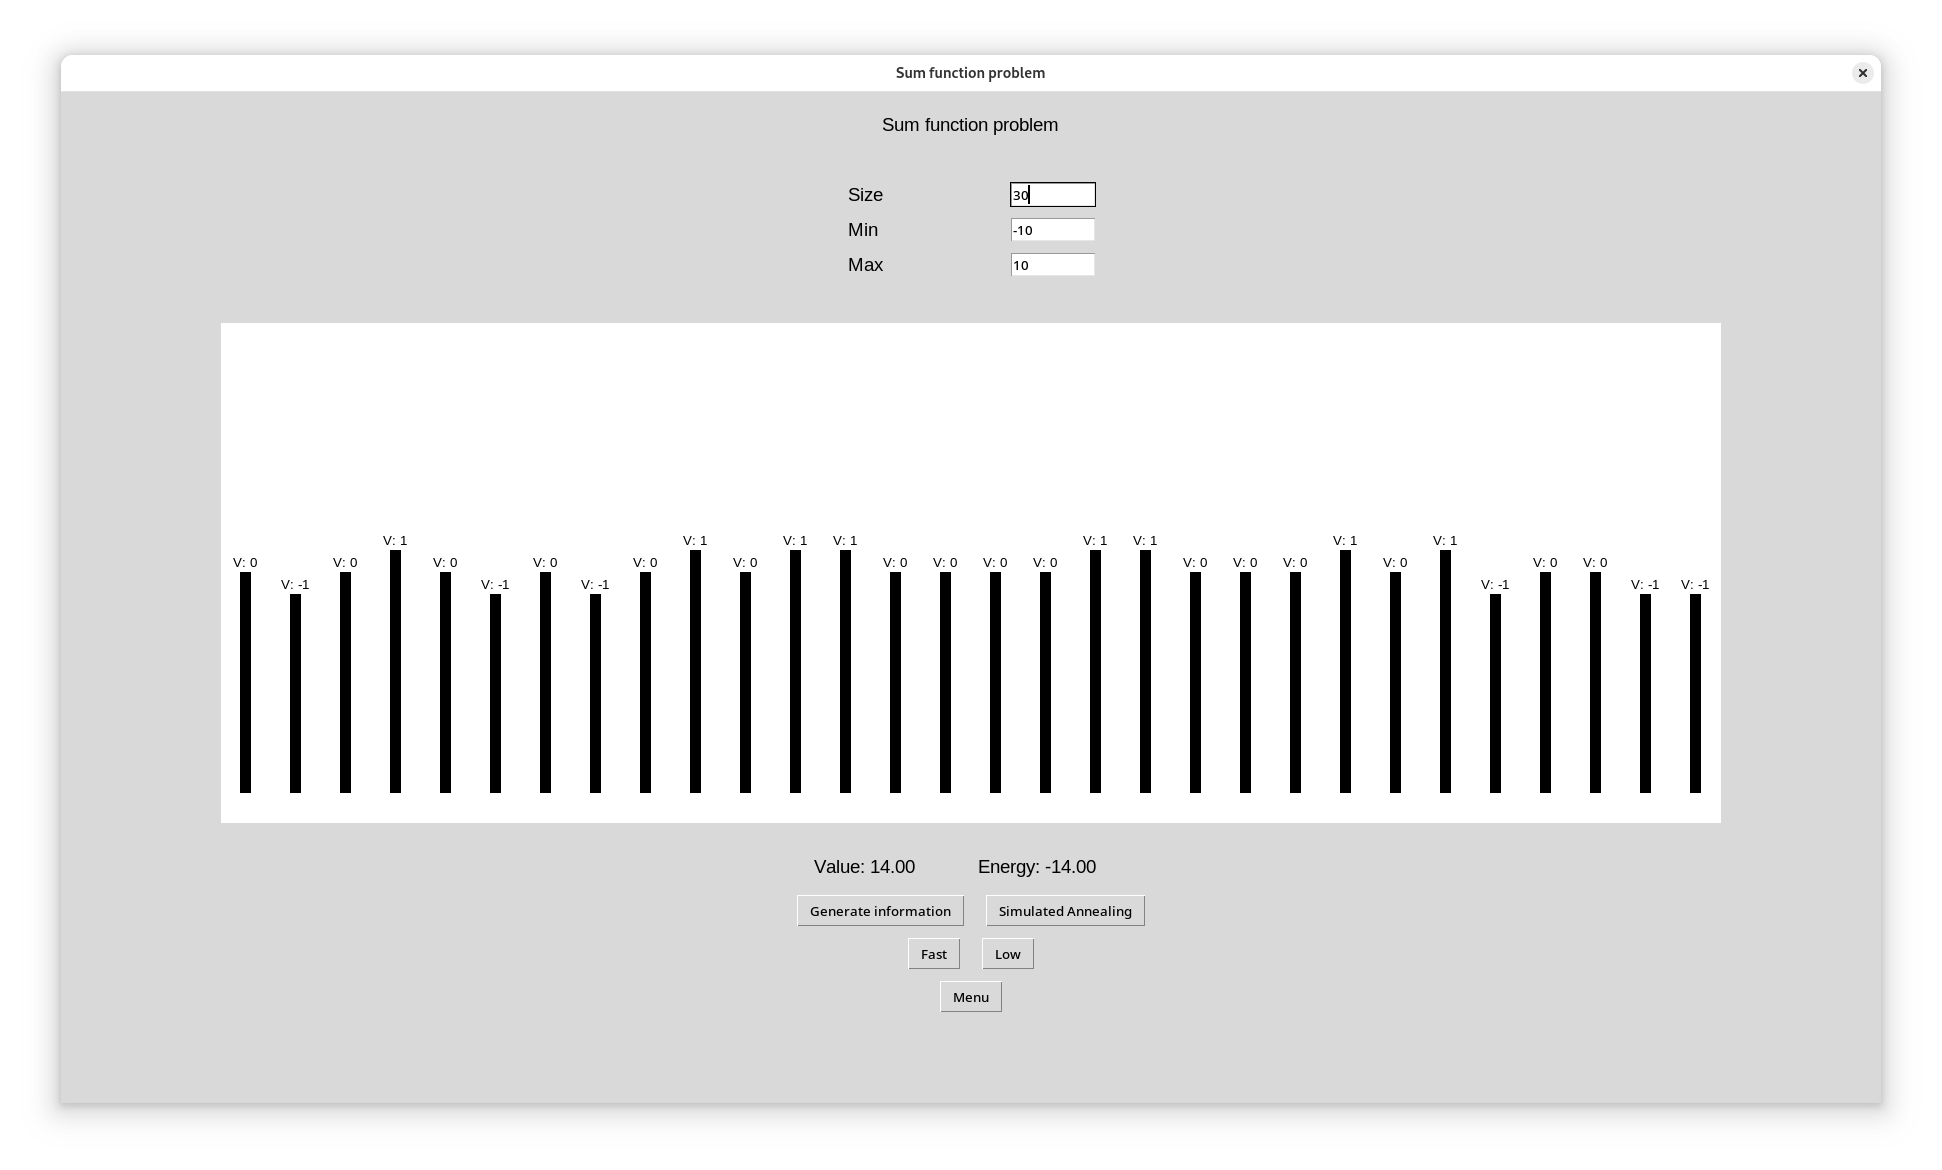
\includegraphics[width=\linewidth]{img/sfp}
	\caption{Sum Function Problem Interface}
	\label{fig:sfp}
\end{figure}

\subsection{CEC 2017}

\section{Metaheuristic}

\subsection{Genetic Algorithm}

\subsection{Selection functions}

\subsection{Crossover functions}

\subsection{Mutation functions}

\subsection{Replace functions}

\begin{lstlisting}[style=pythonstyle, label={lst:sa} ,caption={Constructor de la clase SimulatedAnnealing}]
\end{lstlisting}
